\documentclass[12pt]{article}


\usepackage[dvips,letterpaper,margin=0.75in,bottom=0.5in]{geometry}
\usepackage{cite}
\usepackage{slashed}
\usepackage{graphicx}
\usepackage{amsmath}
\usepackage{braket}
\begin{document}

\title{Chi-Squared Metric and Least Squares Fitting}
\author{Michael Mulhearn}

\maketitle

\section{The $\chi^2$ Metric}
Presented with a series of $N$ measurements:
\begin{displaymath}
\{x_1 \pm \sigma_1, x_2 \pm \sigma_2, ..., x_N \pm \sigma_N\}
\end{displaymath}
we are often concerned with how consistent these results are with a corresponding theoretical prediction:
\begin{displaymath}
\{X_1, X_2, ..., X_N\}
\end{displaymath}
Assuming Gaussian uncertainties for each measurement x, then the probability of one particular measurement is just a Gaussian PDF:
\begin{displaymath}
P_i = \frac{1}{\sqrt{2\pi} \sigma_i} \exp\left(-\frac{1}{2} \frac{(x_i-X_i)^2}{\sigma_i^2}\right)
\end{displaymath}
The probability of the complete set of measurements is called the {\em Likelihood} and it is just the product of the probabilities of each measurement:
\begin{displaymath}
\mathcal{L} = \prod_i P_i = \prod_i \frac{1}{\sqrt{2\pi} \sigma_i} \exp\left(-\frac{1}{2} \frac{(x_i-X_i)^2}{\sigma_i^2}\right)
\end{displaymath}
Since sums are generally easier than products, we consider:
\begin{displaymath}
\log \mathcal{L}
\end{displaymath}
And since physicist think about minimization rather than maximization (pessimists?  gravity?) we take:
\begin{displaymath}
-\log \mathcal{L}
\end{displaymath}
And since there is an annoying factor of $1/2$ in the exponent, we finally take
\begin{displaymath}
-2 \log \mathcal{L}
\end{displaymath}
which we can calculate as:
\begin{displaymath}
-2 \log \mathcal{L} = -2 \sum_i \log\left( \frac{1}{2 \pi \sigma_i }\right) + \sum_i \frac{(x_i-X_i)^2}{\sigma_i^2}
\end{displaymath}
The first term is a constant that does not depend on the measured and predicted values, only on the precision of the experiment.  The second term, is what we call the $\chi^2$ metric:
\begin{equation}
\chi^2 = \sum_i \frac{(x_i-X_i)^2}{\sigma_i^2}
\end{equation}
When $\chi^2$ is small, the measured values $\{x_i\}$ are relatively close to the predicted values $\{X_i\}$ as defined by the experimental uncertainties.  When $\chi^2$ is large, the predicted values are well outside the experimental uncertainties of the measurements.

\section{Maximal Likelihood Method}

Often, we are interested to know which particular parameters of a model maximize the likelihood
of the data we have collected.  For instance, suppose we made $N$ measurements:
\begin{displaymath}
\left\{ x_1 \pm \sigma, x_2 \pm \sigma, ..., x_N \pm \sigma \right\}
\end{displaymath}
of the same quantity, and we would like to find out which single value $X$ is most consistent with these $n$ measurements.  Our $\chi^2$ for this simple model is then:
\begin{displaymath}
\chi^2 = \sum_i \frac{(x_i-X)^2}{\sigma^2}.
\end{displaymath}
We can find the particular value of $X$ that maximizes the likelihood by finding the value that minimizes the $\chi^2$, because $\chi^2 \sim - 2 \log \mathcal{L}$.  We find the minimum from the condition:
\begin{displaymath}
\frac{d\chi^2}{dX} = 0,
\end{displaymath}
which amounts to:
\begin{eqnarray}
0 &=& 2 \sum_i \frac{(x_i-X)}{\sigma^2} \nonumber \\
0 &=& \sum_i x_i - X \sum_i \nonumber \\
X &=& \frac{1}{N} \sum_i x_i \label{eqn:mean}
\end{eqnarray}
which of course is just the mean of the measurements, as expected.

The $\chi^2$ formalism is quite general.  Suppose at each position $x_i$ we make a measurement $y_i$ which has a corresponding theoretical prediction $f(x_i; a, b)$ where $a$ and $b$ are parameters of the theory.  In this case, the $\chi^2$ is given:
\begin{displaymath}
\chi^2 = \sum_i \frac{(y_i-f(x_i,a,b))^2}{\sigma_i^2}
\end{displaymath}
and to determine the best fit values for $a$ and $b$ we would require:
\begin{eqnarray*}
\frac{d\chi^2}{da} &=& 0 \\
\frac{d\chi^2}{db} &=& 0 
\end{eqnarray*}
We can accommodate any number of theory parameters in this fashion.  And the interpretations of $x$ and $y$ are endless.  We can imagine taking measurements of the voltage at particular times, measuring the electric field strength at particular radii, the number of cars produced in a factory each month, and so on.

{\bf Exercise} Calculate a general solution for the best fit parameters of the straight line fit $f = a x + b$.

\section{Interpretation of $\Delta \chi^2$}

Suppose at particular points $\{x_i\}$ we have made measurements $\{y_i \pm \sigma_i\}$ with corresponding theoretical predictions $f(x_i, a)$.  Using the $\chi^2$ formalism we can determine the best fit value $a_0$ for the parameter $a$.  But this is of very little use unless we can also determine the corresponding uncertainty $\sigma_a$ associated with the best fit value $a_0$.  

One approach is to simply apply propagation of uncertainties to the formula determined by minimizing the $\chi^2$, for instance, Equation~\ref{eqn:mean}.  But this approach can be tedious or even unusable in cases where the $\chi^2$ is minimized numerically and no closed form solution is available.   It is well worthwhile, therefore, to consider an alternative approach, that determines these uncertainties directly from the Likelihood and it's corresponding $\chi^2$ distribution.

Let's consider the Likelihood associated with this series of measurements, and interpret it as a probability distribution function for the random variable $a$:
\begin{displaymath}
\mathcal{L}(a) = \prod_i \frac{1}{\sqrt{2\pi} \sigma_i} \exp\left(-\frac{1}{2} \frac{(y_i-f(x_i,a))^2}{\sigma_i^2}\right)
\end{displaymath}
Assume for the moment that this PDF is a Gaussian distribution, and so can written alternatively
as:
\begin{displaymath}
\mathcal{L}(a) =  \frac{1}{\sqrt{2\pi} \sigma_i} \exp\left(-\frac{(a-a_0)^2}{2\sigma_a^2}\right)
\end{displaymath}
explicitly in terms of the best fit value $a_0$ and the uncertainty $\sigma_a$.  The $\chi^2$ is then simply:
\begin{equation} \label{eqn:chisqa}
\chi^2(a; a_0, \sigma_a) = \frac{(a-a_0)^2}{\sigma_a^2}
\end{equation}
We see that:
\begin{displaymath}
\frac{d\chi^2}{da} = \frac{2 (a-a_0)}{\sigma_a^2} = 0
\end{displaymath}
when $a=a_0$ exactly as expected.  We also see that:
\begin{displaymath}
\frac{d^2\chi^2}{da^2} = \frac{2}{\sigma_a^2}
\end{displaymath}

As shown in Fig.~\ref{fig:chisq} the $\chi^2$ for a Guassian likelihood is a parabola, and so the second derivative {\em evaluated anywhere} yields a term containing the uncertainty $\sigma_a$.  However, the region near the minimum of any $\chi^2$ can distribution can be approximated as a parabola about the minimum, and so for a general $\chi^2$ distribution, we have:
\begin{equation} \label{eqn:chisqunc}
\sigma_a^2  = \frac{2}{\left. \frac{d^2\chi^2}{da^2} \right|_{a_0}}
\end{equation}

\begin{figure}[htbp]
\begin{center}
{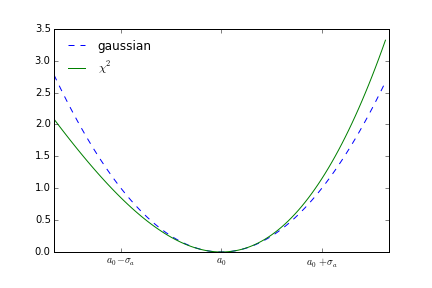
\includegraphics[width=0.75\textwidth]{figs/chisq.png}}
\end{center}
\caption{\label{fig:chisq} Approximation of $\chi^2$ near minimum.}
%x = np.arange(0,10,0.1)
%y = (x - 5)**2/3**2
%z = y + 0.05*(x - 5)**3/3**2 
%plt.plot(x,y,"--",label="gaussian")
%plt.plot(x,z,"-",label="$\chi^2$")
%plt.legend(loc=2,frameon=False)
%plt.xticks([2,5,8],["$a_0 - \sigma_a$", "$a_0$", "$a_0 + \sigma_a$"])
%plt.savefig("chisq.png")
\end{figure}

{\bf Exercise} Show that at the minimum, varying a parameter by it's uncertainty changes the $\chi^2$ by 1.

\section{Numerical Least Squares Fitting}

The $\chi^2$ formalism lends itself easily to numerical solutions, since the problem amounts to the optimization problem of finding the minimum of a function.  A popular approach is the gradient descent approach.  The minimum is approached in steps, with the gradient calculated at each step, and used to point the direction of the next step.  The size of the step can be chosen so that the gradient is approximately constant during the step, such as by estimating the second derivative.  Once at the minimum, the uncertainties can be estimated from the second derivative according to Equation~\ref{eqn:chisqunc}.

The major limitation of the steepest descent approach is that it will generally find only the nearest {\em local} minimum.  There is no guarantee that the global minimum has been reached.  This limitation is generally avoided by making an initial guess which is known to be near the actual minimum.  Also, the results of fits should always be evaluated to make certain they are sensible... local minimums that are not the absolute minimum almost always look ridiculous when plotted against the data!

A complete example implementing a straight line fit in scientific python is included below.  Note a few snippets in particular:
\begin{verbatim}
def func(x, a, b):
    return a*x + b
popt, pcov = curve_fit(func, x, y, sigma=yunc, p0=[1,1],absolute_sigma=True)
\end{verbatim}
The fit function is the user defined function "func", which in this case, takes two parameters ($a$ and $b$).  The call to curve\_fit is where the actual fit is performed.  Notice that the uncertainties are provided explicitly, the initial guesses are provided, and the uncertainties are specified as absolute.

The default behavior of curve\_fit is rather unscientific and intended for the general public.  It simply assumes all uncertainties are equal (if sigma is unspecified) and scales the uncertainties by an amount that gives a reasonable $\chi^2$ at the minimum.  This is seldom what a physicists wants.

You obtain the fitted parameters and their uncertainties from the return values of the functions:
\begin{verbatim}
# report the fitted values:
print "fitted values:  ", popt

# report the uncertainties, determined from the diagonals of the covariance matrix:
perr = np.sqrt(np.diag(pcov))
print "statistical uncertainties:  ", perr
\end{verbatim}
The non-diagonal elements are beyond the scope of this course, but generally provide information about how the fit parameters are correlated.  Generally speaking, highly correlated parameters should be avoided by choosing a more appropriate parameterization.

The full example is here:

\begin{verbatim}
#
# fiteg.py
#
# An example program for fitting a straight line to data with uncertainties:
# 

import matplotlib.pyplot as plt
import numpy as np
from scipy.optimize import curve_fit

# generate simulated data y = a*x + b according to:
a = 3;
b = 5;
x = np.arange(0,10)
y = a*x + b
yunc = 0.5 + y*0.03
# smear data by the uncertainties yunc
y = y + np.random.normal(scale=yunc)

# plot the simulated data with uncertainties:
fig, ax = plt.subplots(1,1)
ax.set_xlabel('x')
ax.set_ylabel('y')
ax.errorbar(x,y,yunc,fmt="ko")

# fit the data to the straight line implemented in "func":
# note we provide explicitly:
# - the uncertanities on y (sigma = yunc)
# - the starting guess for our parameters (p0=[1,1])
# - we specify the sigmas are absolute, not just relative, when determining statistical 
#   uncertainties (absolute_sigma=True)  A good test is to set this False and make 
#   certain it doesn't dramatically change your results, which would be evidence that 
#   either your uncertainties are inaccurate or the model is poor.

def func(x, a, b):
    return a*x + b
popt, pcov = curve_fit(func, x, y, sigma=yunc, p0=[1,1],absolute_sigma=True)

# report the fitted values:
print "fitted values:  ", popt

# report the uncertainties, determined from the diagonals of the covariance matrix:
perr = np.sqrt(np.diag(pcov))
print "statistical uncertainties:  ", perr

# report the pulls (measured - true value) / uncertainty.  (which should folow unit 
# Guassian distribution, i.e. typical values are ~ +/- 1)
pull = (popt-np.array([a,b]))/perr
print "pulls from fit:  ", pull

# plot the fitted line along with the data:
ax.plot(x,func(x,*popt),"--")
plt.show()
\end{verbatim}


%\newpage
%\section{Exercises}

%\noindent
%{\bf Problem 1:} Show that...\\

%\vskip 1cm
%\noindent
%{\bf Problem 2:} Show that...\\


\end{document}




